% example with several commonly used tex constructs
\section{Section}

Example citation \cite{CBM-stat-rep}. Entry must be in
dabc-bibitems.tex.\\ % new line

Example figure
\begin{figure}[htb]
\centering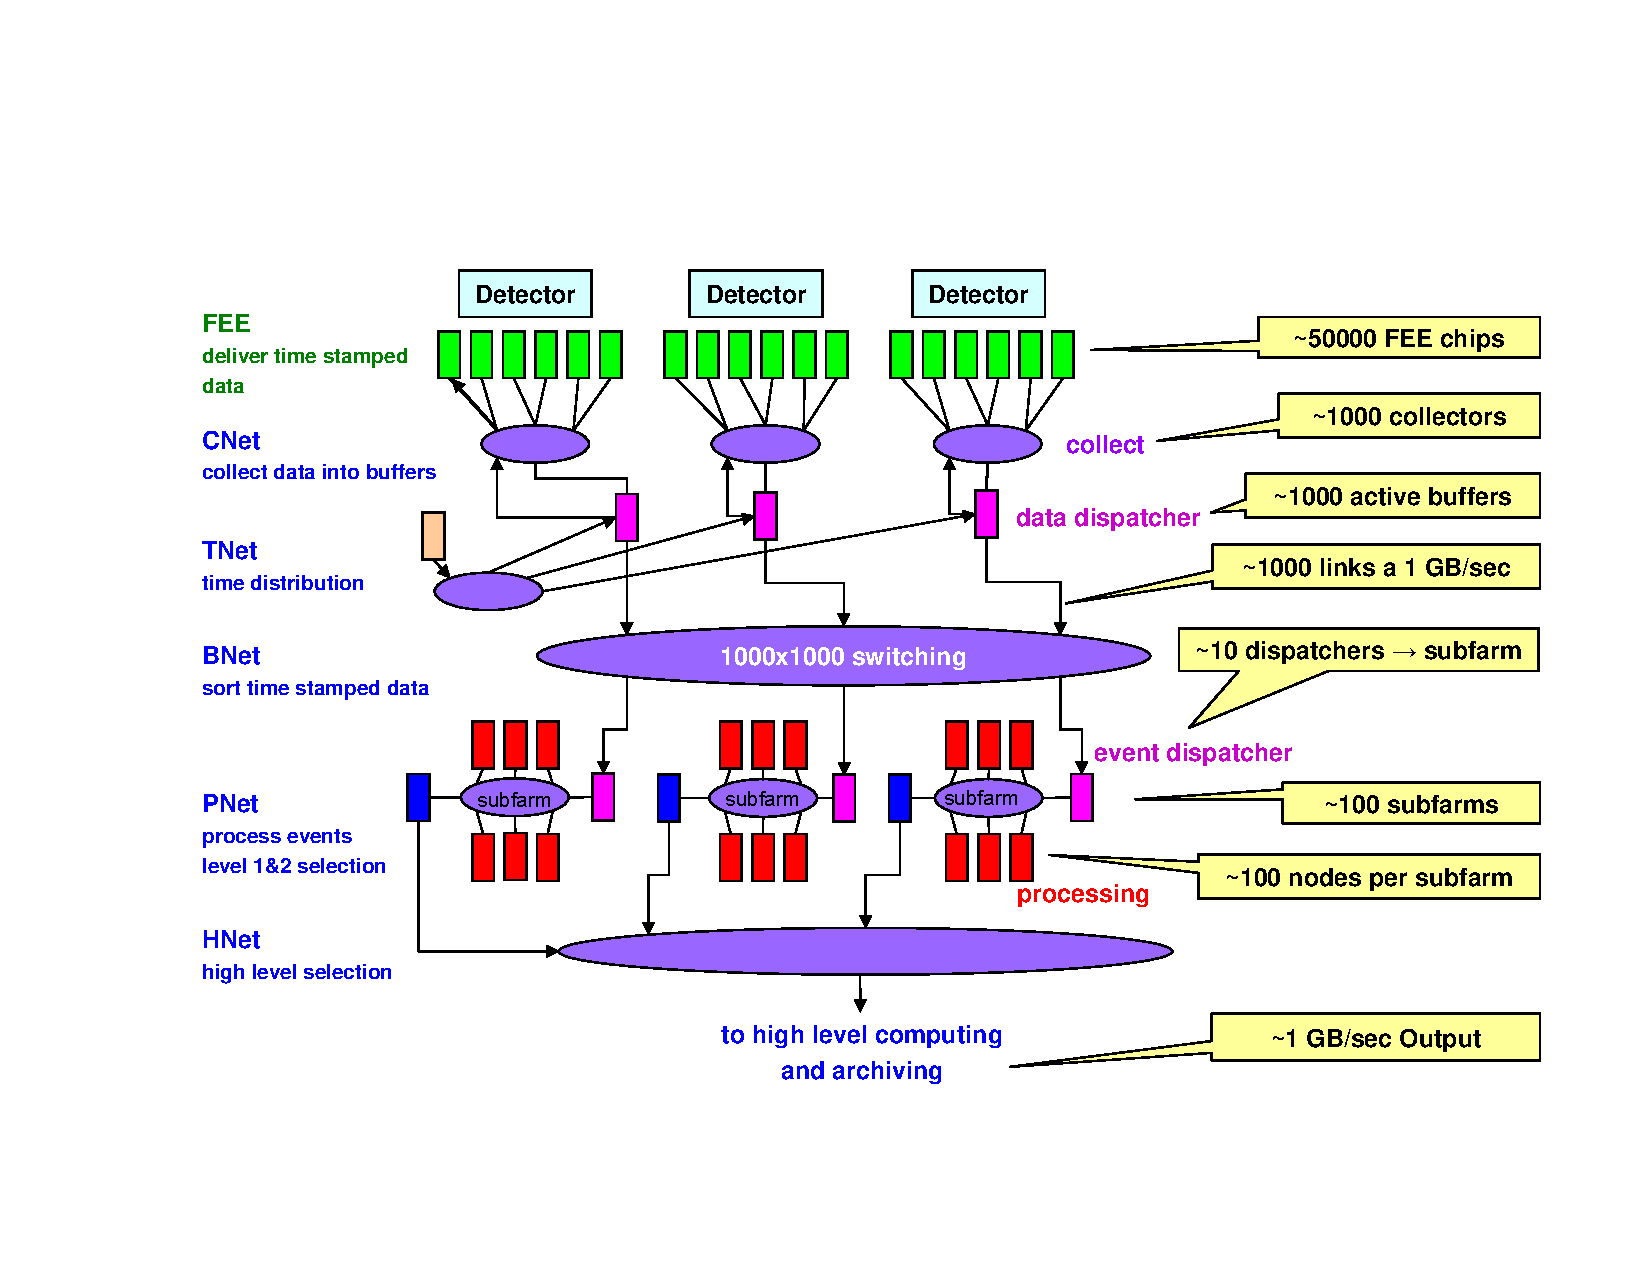
\includegraphics[angle=-90,width=.8\textwidth]{dabcf-daq-all} % pdf file
\caption{CBM overall data processing architecture}
\label{fig:user-fig} % give it a name for references
\end{figure}

\index{Demonstrator!mission} % entry in index

Reference to Fig.~\ref{fig:user-fig}.
\clearpage % new page

\section{Next section}
\index{Demonstrator!mission} % entry in index

% define a marker to be referenced from outside:
\hyperdef{user}{name}{[Marker:user:name]}\\
% Reference to external paper having a \hyperdef{sw}{data}
See also \hyperref{http://www-linux.gsi.de/~mbs/main-software.pdf}{sw}{data}{Software paper}.\\
See also \hyperref{http://www-linux.gsi.de/~mbs/main-intro.pdf}{in}{mission}{Introduction paper}.

\subsection{Subsection}
\index{Demonstrator!technology} % entry in index

Example of a compact list with bullets
\begin{compactitem}[$\bullet$]
\item FEE: self-triggered, data push, conditional RoI based readout
\item CNet: combined data, time, control, and RoI traffic
\end{compactitem}

Another compact list with circles
\begin{compactitem}[$\circ$]
\item Hardware
\item Firmware
\end{compactitem}
\subsubsection{Subsubsection}

Example of compact description list
\begin{compactdesc}
\item[Hardware] There are mainly three boards with different tasks but similar architecture.
\item[Data formats] The data and time stamp formats must be defined early because they are
interpreted at many occasions. A change would have big impact.
\end{compactdesc}

Example of compact numerated list
\begin{compactenum}
\item compressed
\item coded geographical address
\end{compactenum}

Example of table
\begin{table}[h]
\begin{tabular}{|p{2.0cm}|p{2.0cm}|p{3.0cm}|p{1.6cm}|p{5.0cm}|}      \hline
Document   & Date        & Editor       & Revision & Comment      \\ \hline
DABC-user & 2008-12-18 & Hans G.Essel & 1.0.0      & First scetch \\ \hline
\end{tabular}
\caption{Example of table.}
\label{user-table}
\end{table}
